\documentclass[a4paper]{vanvliet_paper}

% WIP title
\title{Beamformer Study}

% Author list
\author[1*]{Britta U. Westner}
\author[2,3*]{Christian Kiefer}
\author[4]{Marijn van Vliet}
\affil[1]{Center of Functionally Integrative Neuroscience, Department of Clinical Medicine, Aarhus University}
\affil[2]{Institute of Neuroscience and Medicine, Forschungszentrum Jülich GmbH}
\affil[3]{RWTH Aachen University}
\affil[4]{Department of Neuroscience and Biomedical Engineering, Aalto University}
\affil[*]{Shared first authorship}

% List of acronyms we use in the paper
\newacronym{EEG}{eeg}{electroencephalography}
\newacronym{MEG}{meg}{magnetoencephalography}
\newacronym{fMRI}{\textnormal{f}mri}{functional magnetic resonance imaging}
\newacronym{EMG}{emg}{electromyography}
\newacronym{EOG}{eog}{electro-oculogram}
\newacronym[\glslongpluralkey={event-related potentials}]{ERP}{erp}{event-related potential}
\newacronym{LCMV}{lcmv}{linearly constrained minimum variance}
\newacronym{DICS}{dics}{dynamic imaging of coherent sources}


% Bibliography file
\addbibresource{references.bib}

% Indicate that this is a draft
\draft

% Add line numbers
\linenumbers

% Ok, let's go!
\begin{document}
\maketitle

\begin{abstract}
    We evaluate the effect of various parameters on beamformer source estimation.

    \begin{keyword}
        beamformer \sep LCMV \sep DICS \sep model evaluation \sep simulation \sep MEG
    \end{keyword}
\end{abstract}

\section{Introduction}

There is a beamformer called \gls{LCMV}\cite{VanVeen1997}.
The \gls{LCMV} produces a really nice result (\autoref{fig:result}).
There is also a beamformer called \gls{DICS}\cite{Gross2001}.

\begin{figure}[h]
    \centering
    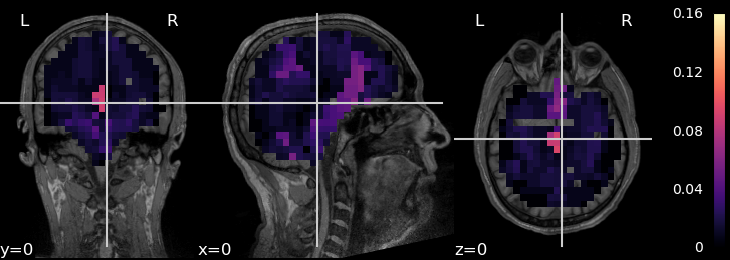
\includegraphics[width=10cm]{figures/figure1.png}
    \caption{The localization error for the \gls{LCMV} beamformer when using the default parameter settings.}\label{fig:result}
\end{figure}

\section{Methods}
\section{Results}
\section{Discussion}
\section{Conclusions}

\section{Acknowledgements}

MvV is supported by the Academy of Finland (grant 310988).

\printbibliography{}

\end{document}
